

\chapter{Preliminaries}

In this chapter, we intend to provide the technical and theoretical background for the terms we use in the thesis. We describe datasets used for evaluations, explain some technical terms later used, and provide a quick overview of Deep Neural Networks.

\section{Distance Metrics}

In our solutions presented we order the database of items based on their similarity/distance to the query. We use cosine distance and euclidean distance. We experiment with those metrics, based on the disadvantages of the euclidean distance in higher dimensionality spaces.

\subsection{Cosine Distance}

We use following version of cosine distance based on the cosine similarity.

\begin{equation}
\text{similarity} = \cos ({\bf p},{\bf q})= {{\bf p} {\bf q} \over \|{\bf p}\| \|{\bf q}\|} = \frac{ \sum_{i=1}^{n}{{\bf p}_i{\bf q}_i} }{ \sqrt{\sum_{i=1}^{n}{{\bf p}_i^2}} \sqrt{\sum_{i=1}^{n}{{\bf q}_i^2}} }
\end{equation}

\begin{equation}
    \text{cos\_distance} = 1 - \text{similarity}
\end{equation}

\subsection{Euclidean Distance}
\begin{equation}
d(p, q) = \sqrt{\sum_{i=1}^n (p_i - q_i)^2}    
\end{equation}

\section{Dataset}

We use Vimeo Creative Commons Collections (V3C1)\footnote{\href{https://www-nlpir.nist.gov/projects/tv2019/data.html}{TRECVID 2019 Video Data}} dataset for experimenting and evaluations. The dataset is composed of 7475 Vimeo videos. We selected only the first 750 videos for proving concepts of our work. From these 750 videos, we used an extraction tool from VIRET \cite{lokovc2019framework}. After extraction, we obtained 111\ 764 images from 750 videos with resolution 320x180.

The videos capture a wide range of sceneries on many different occasions. We can see many different landscapes, from seas to mountain views, from desert to snow. A large proportion of the videos contain people. Videos capture people doing different activities, i.e., from Hindi wedding to skateboarding in a park or a news broadcast.

\subsection{Collages used for evaluation}

In the chapter \ref{ch:object_location} we do different evaluations of proposed systems. To do that in a known-search item task, we beforehand annotated a set of the data. The data consist of 100 collages, all containing a visual image description of a given scene. The average size of the images used in the collages covers 15\% of the canvas. Five \% of the dataset consists of images bigger than 80\% of the canvas. We provide visualization of the distribution of the annotated queries in figure \ref{fig:annotated_dataset}.

For the annotation, we used our application used for spatial queries. It is possible to save the collage by clicking "Submit Collage." The average time spends on annotation one image was 91 seconds. This time includes searching for images online, pasting them onto the canvas, and usually also waiting for the query to go through. The majority of the time is spent by looking for a good match in the image search engine.

\begin{figure}
     \centering
     \begin{subfigure}[b]{0.48\textwidth}
         \centering
         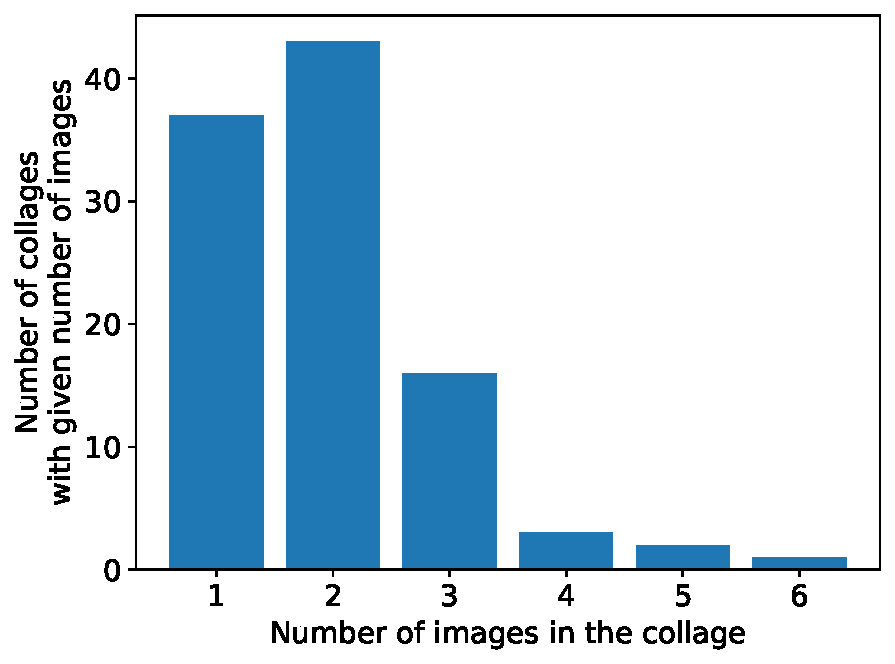
\includegraphics[width=\textwidth]{graphs/num_queries_in_request.pdf}
         \caption{Number of images on a canvas for a collage.}
         \label{fig:y equals x}
     \end{subfigure}
     \hfill
     \begin{subfigure}[b]{0.48\textwidth}
         \centering
         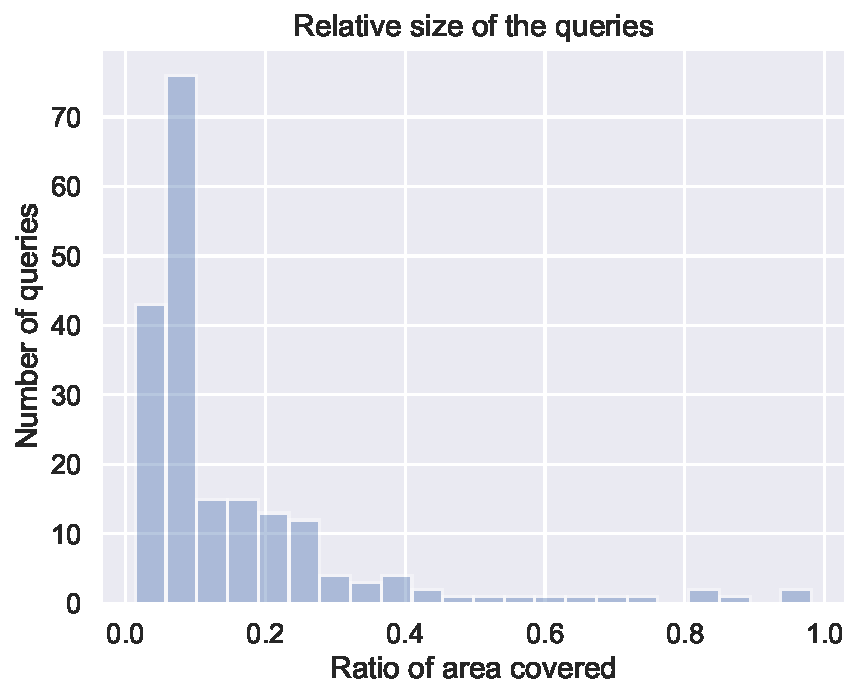
\includegraphics[width=\textwidth]{graphs/queries_size.pdf}
         \caption{Size of the canvas which is covered by a query image.}
         \label{fig:three sin x}
     \end{subfigure}
    
    \caption{Annotated collages properties}
    \label{fig:annotated_dataset}
\end{figure}


\section{Intersection over Union}

In the following chapters, we use Intersection over Union (IoU) as a characteristic of overlapping. Intersection over Union (also known as Jaccard index\footnote{\href{https://en.wikipedia.org/wiki/Jaccard_index}{https://en.wikipedia.org/wiki/Jaccard\_index}}) measures similarity between two sets. We use it as a metric to express how much two regions (i.e., two rectangles) overlap. 

The definitions of the Interectio over Union is as follows:
$$
    J(A, B) = 
    \begin{cases}
      1, & \text{if\ A and B are empty} \\
      \frac{|A \cap B|}{|A \cup B|}, & \text{otherwise}
    \end{cases}
$$

In our case, the $|A \cap B|$ represents the are belonging to both regions. The  $|A \cup B|$ represents the area covered by union of the both regions. A visual representation of the fomrula is displayed in the Figure \ref{fig:intersection_over_union}.

\begin{figure}
    \centering
	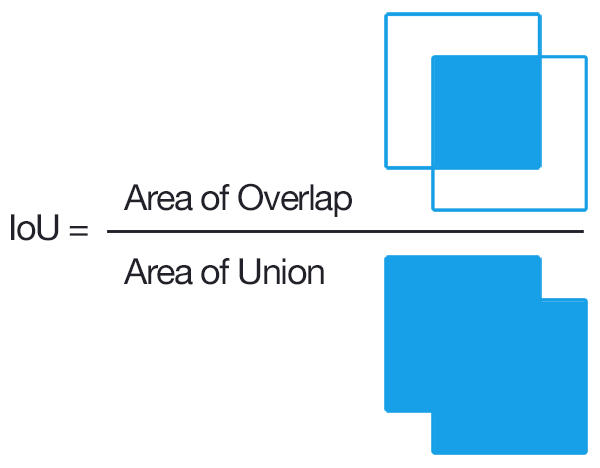
\includegraphics[width=0.3\linewidth]{img/Intersection_over_Union_-_visual_equation.png}
	\caption{Intersection over Union between regions. Source: Wikipedia, CC BY-SA 4.0}
	\label{fig:intersection_over_union}
\end{figure}


\section{Deep Neural Networks}

In recent years we witnessed many records-breaking new machine learning models. Many of those were possible, thanks to the advancement of Deep Neural Networks (DNN). Nowadays, these models replaced more traditional Machine Learning approaches in many tasks.

Deep Neural Network is a machine learning model, whose goal is to approximate a given function \(f\). The set of parameters is often referred to as \(\theta\). One of the everyday tasks performed by these networks is classification, where the goal of the network is to predict which category sample \(X\) belongs. Even though we will not perform a classification task in this thesis, we will use some of the available classification networks.

When we talk about neural networks, we usually refer to feedforward network. These networks consist of set of the layers, where information during the evaluation is passed only in one direction. This can be imagined as an applying a function on the results from the previous layer. In example, let's create a small neural network. Denote first layer as \(f_1\) and second layer as \(f_2\). The output of the network will be \(f_2\left(f_1\left(\right)\right)\).

Stacking more and more layers on top of each other lead us to a notation \emph{deep} neural networks. This notation has no fixed threshold on which networks "deserve" to be called deep, therefore we do not recognise any importance to the naming "deep". 

The first and last layer are commonly refferences as \emph{input} and \emph{output} layer. Layers between input and output layer are usually denoted as \emph{hidden} layers. Deep neural networks can have four or hundreds layers and each layer of the layer can have even unique structure. \emph{Network Architecture} captures the "build order" of the network. It is important to note, that there exist many networks with different architectures solving the same task.

There are many reasons for advancement of neural networks in the past years. One of the crucial stones were not only theoretical innovations used for the networks but increasing computablity limits. Deep Neural Networks \emph{learn} to approaximate function by \emph{training}. This training is usually the heaviest part of the computation. Even though, it is enough to usually train once and use forever, it still lay some limitations on the size of the networks or the functions used.

Since this topic is wide, we recommend more thorough reading for example in Neural Networks and deep learning online book\footnote{http://neuralnetworksanddeeplearning.com/}.

\subsection{Convolution Neural Networks}

Convolution Neural Networks (CNN) are class of Deep Neural Networks. Even though the primes of convolutional neural netwroks date back to late 1980s (\cite{lecun1989backpropagation}), it took another 20 years for further advancements in the research area. Convolution Neural Networks are mainly used in image-related tasks, such as image classification ("What is on the image?"), object detection ("Where are the objects in the image and what are they?") or even content generation ("Create a new image"). Their abilities were also tested in many not image related tasks, i.e. music genre recognition.

Convolution Neural Networks are specialized kind of networks which work with grid-like topology. For 1D can be example as time-series, or for 2D most typically image pixels represent a grid. The name \emph{convolution} refers to using a mathematical linear function \emph{convolution} in at least of the layers. Simplificated overview of the structure is displayed in figure \ref{fig:convolution_neural_network}. We refer to \cite{Goodfellow-et-al-2016} for more understanding of \emph{convolutional layers}.

\begin{figure}
    \centering
    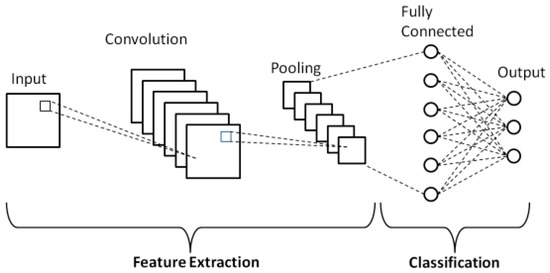
\includegraphics[width=0.98\textwidth]{img/convolution_neural_network.jpg}
    \caption{Schematic diagram of a basic convolution neural networks. Source: Phung, V.H.; Rhee, E.J. A High-Accuracy Model Average Ensemble of Convolutional Neural Networks for Classification of Cloud Image Patches on Small Datasets. Appl. Sci. 2019, 9, 4500.}
    \label{fig:convolution_neural_network}
\end{figure}

\subsection{Transfer Learning}

Transfer Learning is a research problem in machine learning that focuses on storing knowledge gained while solving one problem and applying it to different problem. We have seen many successful transfers not only of the netwroks architecture but also parameters learned to a new task. This helps us to reduce the cost of the training and often also to overcome unsufficient set of training examples for the new task.

We utilise some of the pretrained Convolution Neural Networks. Networks we use are mostly pretrained on \emph{ImageNet}\footnote{http://www.image-net.org/}. ImageNet served as a benchmark for comparing the performance of the different networks. Since the ImageNet is a mainly classification task, we utilize the transfer learning in a way to obtain deep features. This can be done by working with layers close to the end of the networks. These layers already contain encoded information about the image in high dimensional vectors. Our task is to use these deep features obtained for solving our known-search item task.


\begin{figure}
    \centering
	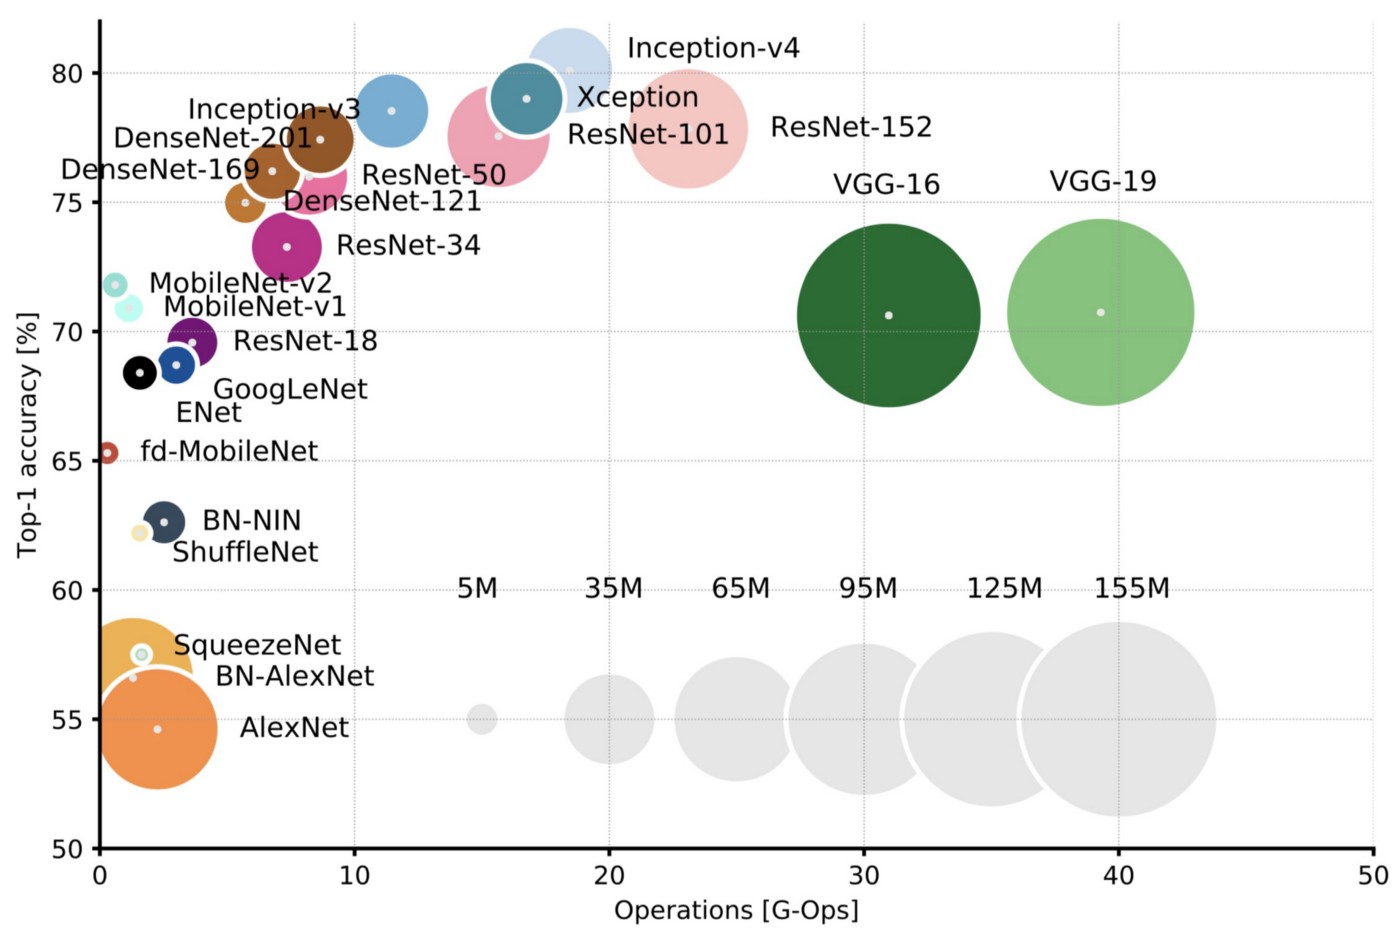
\includegraphics[width=0.8\linewidth]{img/network-comparison.jpeg}
	\caption{Top-1 one-crop accuracy versus amount of operations required for a single forward pass. The size of the blobs is proportional to the number of network parameters. Source: \cite{canziani2016analysis}}
	\label{fig:camera-setup}
\end{figure}

\section{Keras}

Keras (\cite{chollet2015keras}) is a deep learning API written in Python, running on top of the machine learning platform TensorFlow\cite{tensorflow2015-whitepaper}. It was developed with the focus on experimentation in deep learning. We use it and its pretrained models in this thesis. The models available in Keras Applications, which we use, were trained on ImageNet. Keras API allows us to separate the model from last fully connected layer used for classification (since default ImageNet is a classification task). 

\section{Dlib}
Dlib (\cite{king2009dlib}) is a modern C++ toolkit containing machine learning algorithms and tools for creating complex software in C++ to solve real world problems. Some of the modules are provided with Python API. We use Dlib library for a face detection and also face features extraction. For both we use face\_recognition API (\cite{geitgey2016machine}).






% We consider a known set of images I and a query Q∈ I. We utilize a representation ^Q over Q, such that minimize search_rank(^Q, I). We define search_rank as an ordering function based on similarity function (or inverse of distance function). We focus on testing different representations ^Q for query Q.  




